\section{Introduction to Attention Mechanism}
\begin{frame}{}
  \LARGE \textbf{Introduction to Attention Mechanism}
\end{frame}

\begin{frame}{Introduction to Attention Mechanism}
  \textbf{Core Idea:} Let the decoder \textbf{focus on different parts of the input} sequence at each step of decoding.
  \vspace{1em}
  \begin{itemize}
    \item[\textcolor{red}{$\blacktriangleright$}] At each decoding step, compute a \textbf{weighted sum} over all encoder hidden states.
    \item[\textcolor{red}{$\blacktriangleright$}] Weights reflect \textbf{relevance} of each input word to the current output word.
  \end{itemize}
  \vspace{1em}
  \textcolor{teal}{\textbf{``Soft search'' over inputs $\rightarrow$ more context-awareness.}}
\end{frame}

\begin{frame}{Mathematical Formulation of Attention}
  \begin{flushleft}
    \textbf{1. Alignment Score:}
    \begin{equation*}
      e_{t,s} = \text{score}(h_{t-1}^{\text{dec}}, h_s^{\text{enc}})
    \end{equation*}

    \textbf{2. Attention Weights (Softmax):}
    \begin{equation*}
      \alpha_{t, s} = \frac{\exp(e_{t, s})}{\sum_{s'} \exp(e_{t, s'})}
    \end{equation*}

    \textbf{3. Context Vector:}
    \begin{equation*}
      c_t = \sum_s \alpha_{t, s} h_s^{\text{enc}}
    \end{equation*}

    \textbf{4. Decoder Step:}
    \begin{equation*}
      y_t = \text{Decoder}(y_{t-1}, h_{t-1}^{\text{dec}}, c_t)
    \end{equation*}
  \end{flushleft}
\end{frame}

\begin{frame}{Attention Models}
  \centering
  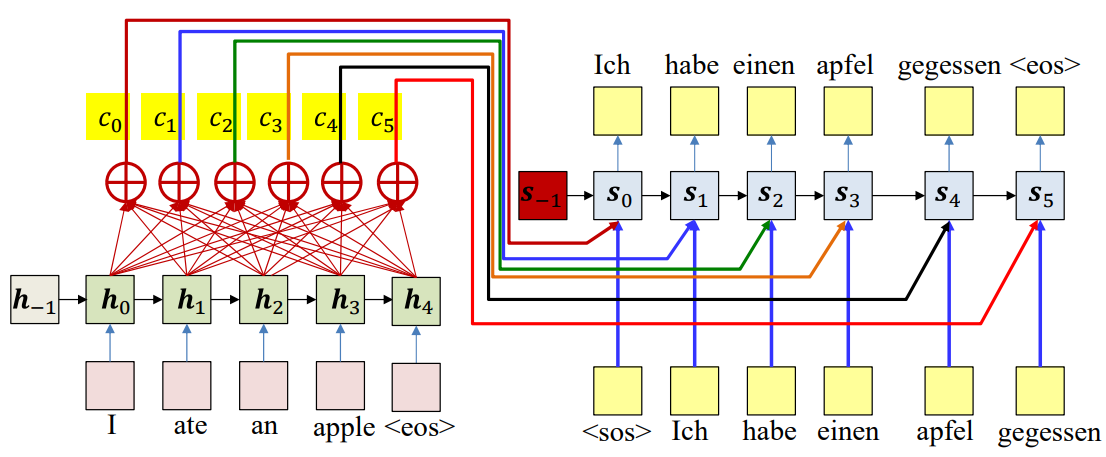
\includegraphics[width=0.4\paperwidth,height=0.4\paperheight,keepaspectratio]{images/seq2seq+attention/seq2seq_attention_context_decoder_states.png}

  {\scriptsize Source: after CMU 11-785 (Spring 2024), Lecture 18: Sequence to Sequence Models \& Attention, slide~28.}
  \begin{itemize}
      \item \textbf{Attention weights:} The weights are dynamically computed as functions of decoder state.
      \item \textbf{Expectation:} if the model is well-trained, this will automatically ``highlight'' the correct input.
      \item But how are these computed?
  \end{itemize}
\end{frame}

\begin{frame}{Attention weights at time $t$}
  \centering
  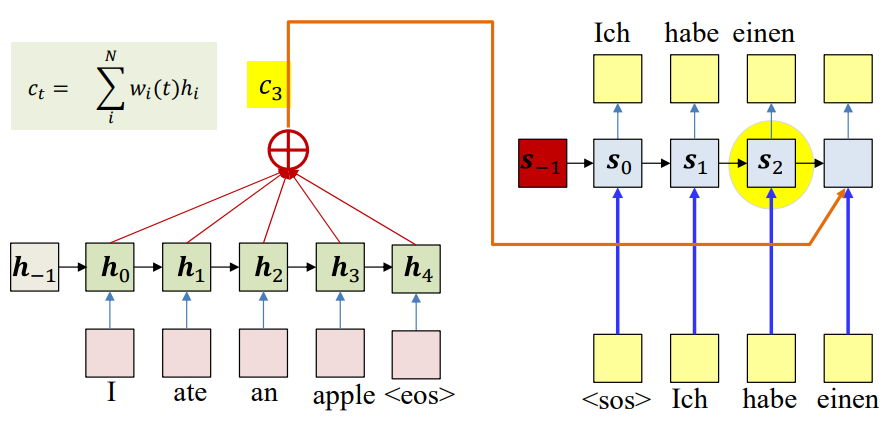
\includegraphics[width=0.4\paperwidth,height=0.4\paperheight,keepaspectratio]{images/seq2seq+attention/seq2seq_attention_weighted_sum_context.png}

  {\scriptsize Source: after CMU 11-785 (Spring 2024), Lecture 18: Sequence to Sequence Models \& Attention, slide~29.}
  \begin{itemize}
      \item The ``attention'' weights $w_i(t)$ must be computed from available information at time $t$.
      \item The primary information is $s_{t-1}$ (the state at time $t-1$).
      \item Also, the input word at time $t$, but generally not used for simplicity.
  \end{itemize}
  \begin{equation*}
      c_t = \sum_{i=1}^N w_i(t) h_i
  \end{equation*}
\end{frame}

\begin{frame}{Requirement on attention weights}
  \centering
  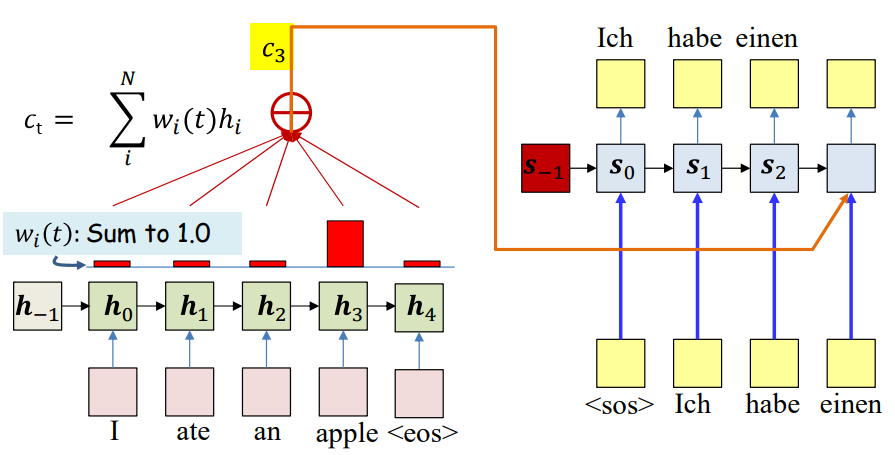
\includegraphics[width=0.4\paperwidth,height=0.4\paperheight,keepaspectratio]{images/seq2seq+attention/seq2seq_attention_weights_distribution.png}

  {\scriptsize Source: after CMU 11-785 (Spring 2024), Lecture 18: Sequence to Sequence Models \& Attention, slide~30.}
  \begin{itemize}
      \item The weights must be positive and sum to 1.0 (i.e., be a distribution).
      \item Ideally, they must be high for the inputs most relevant to the current output and low elsewhere.
      \item \textbf{Solution: A two step weight computation}
      \begin{itemize}
          \item First compute raw weights (which could be +ve or –ve).
          \item Then softmax them to convert them to a distribution.
      \end{itemize}
  \end{itemize}
\end{frame}

\begin{frame}{Requirement on attention weights}
  \centering
  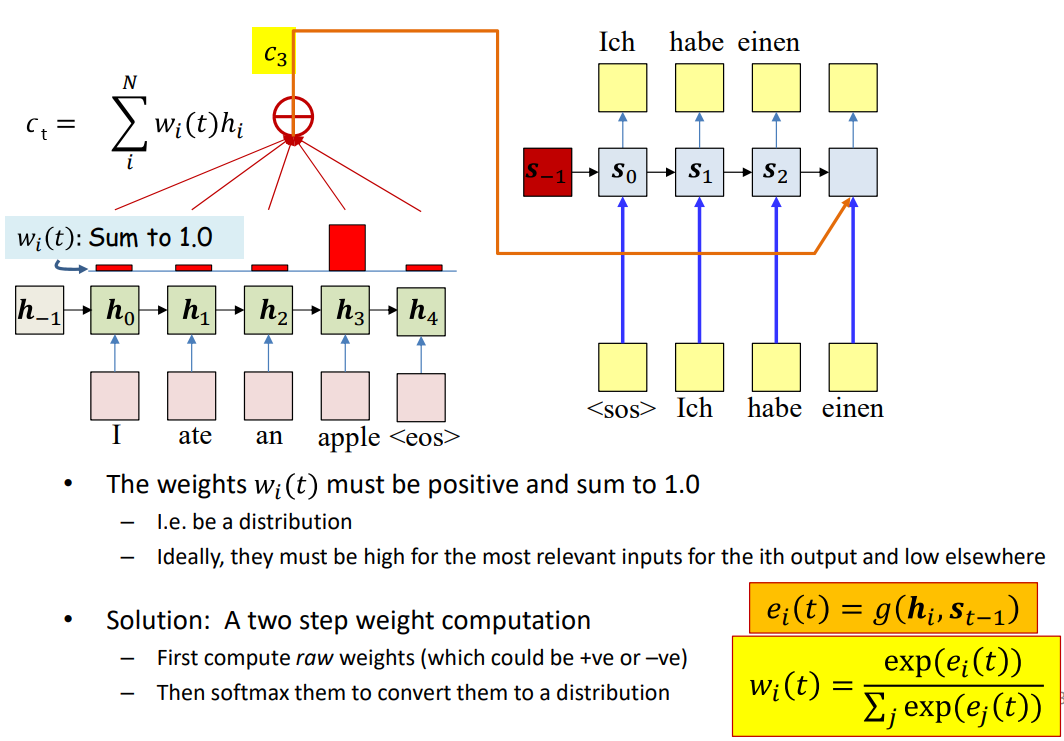
\includegraphics[width=0.8\paperwidth,height=0.66\paperheight,keepaspectratio]{images/seq2seq+attention/seq2seq_attention_weight_softmax_formula.png}

  {\scriptsize Source: after CMU 11-785 (Spring 2024), Lecture 18: Sequence to Sequence Models \& Attention, slide~31.}
\end{frame}

\begin{frame}{Quiz: Attention Framework}
  \begin{enumerate}
      \item The attention framework computes a different ``context'' vector at each output step?
      \item The context vector is chosen as the hidden representation of the word with the highest weight?
      \item The weight is a function of the encoder representation and the most recent decoder state?
  \end{enumerate}
\end{frame}

\begin{frame}{Quiz: Answer}
  \begin{enumerate}
      \item The attention framework computes a different ``context'' vector at each output step? \textbf{True}
      \item The context vector is chosen as the hidden representation of the word with the highest weight? \textbf{False}
      \item The weight is a function of the encoder representation and the most recent decoder state? \textbf{True}
  \end{enumerate}
\end{frame}

\begin{frame}{Requirement on attention weights}
  \centering
  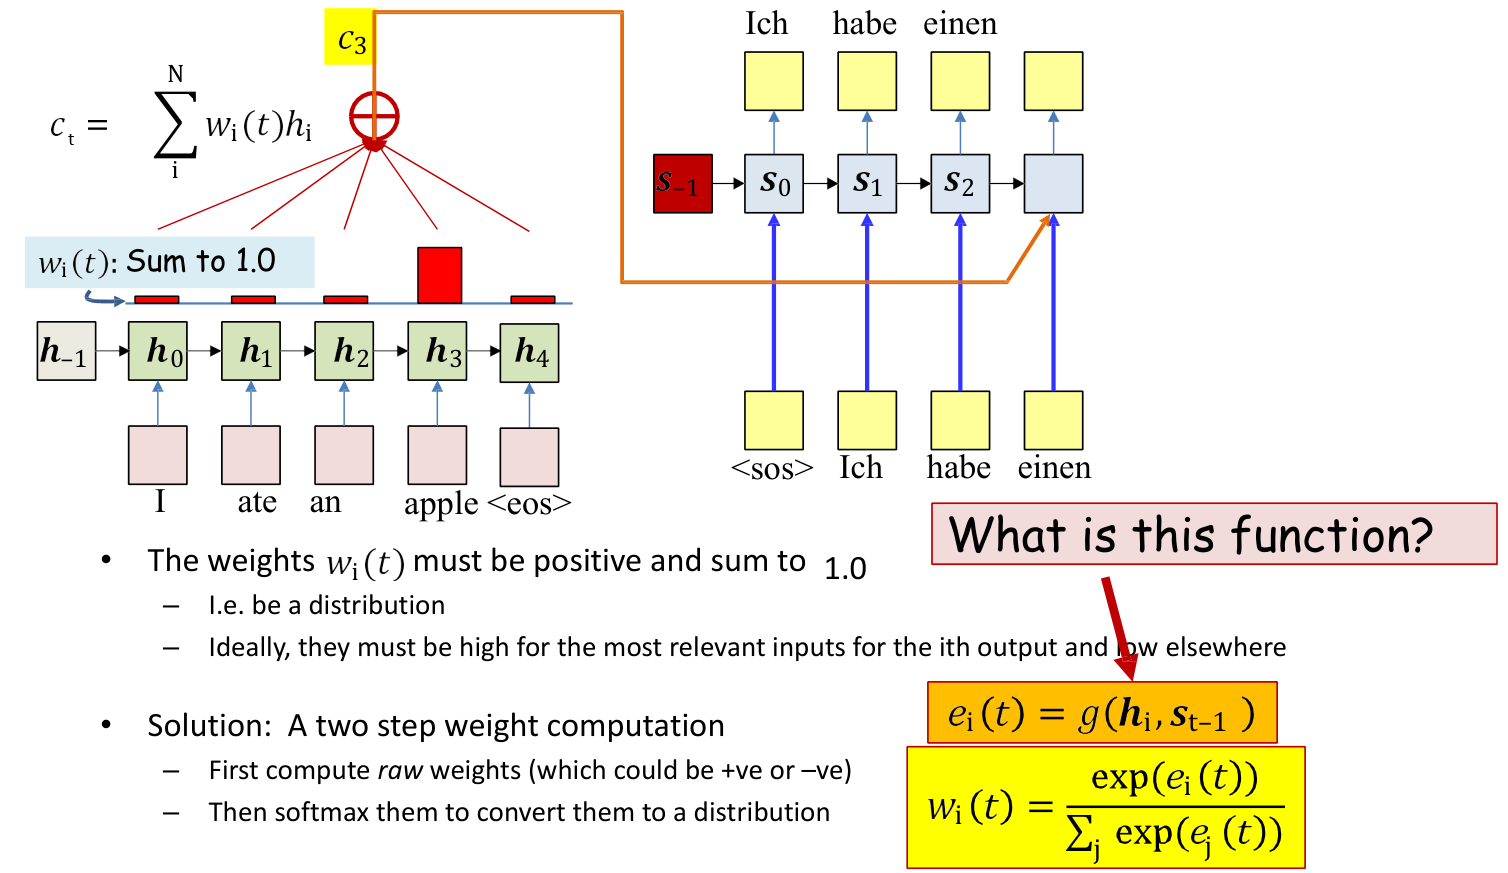
\includegraphics[width=0.8\paperwidth,height=0.66\paperheight,keepaspectratio]{images/seq2seq+attention/seq2seq_attention_scoring_function_question.png}

  {\scriptsize Source: after CMU 11-785 (Spring 2024), Lecture 18: Sequence to Sequence Models \& Attention, slide~34.}
\end{frame}

\begin{frame}{Attention weights}
  \centering
  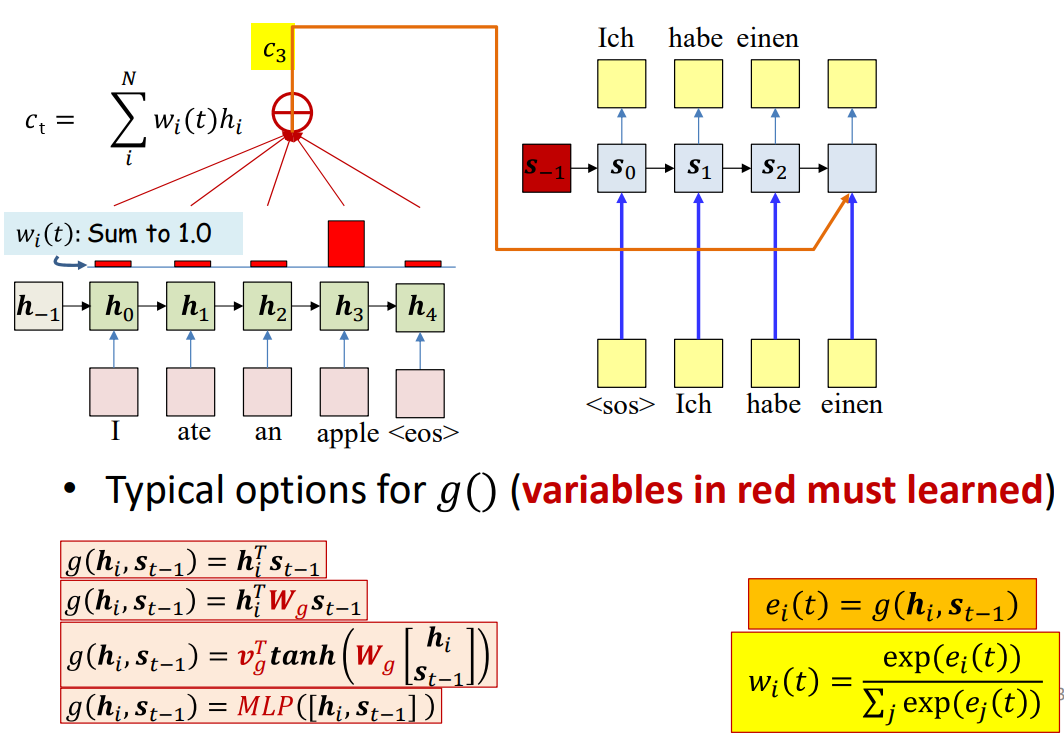
\includegraphics[width=0.8\paperwidth,height=0.66\paperheight,keepaspectratio]{images/seq2seq+attention/seq2seq_attention_scoring_function_options.png}

  {\scriptsize Source: after CMU 11-785 (Spring 2024), Lecture 18: Sequence to Sequence Models \& Attention, slide~35.}
\end{frame}

\begin{frame}{Attention weights}
  \centering
  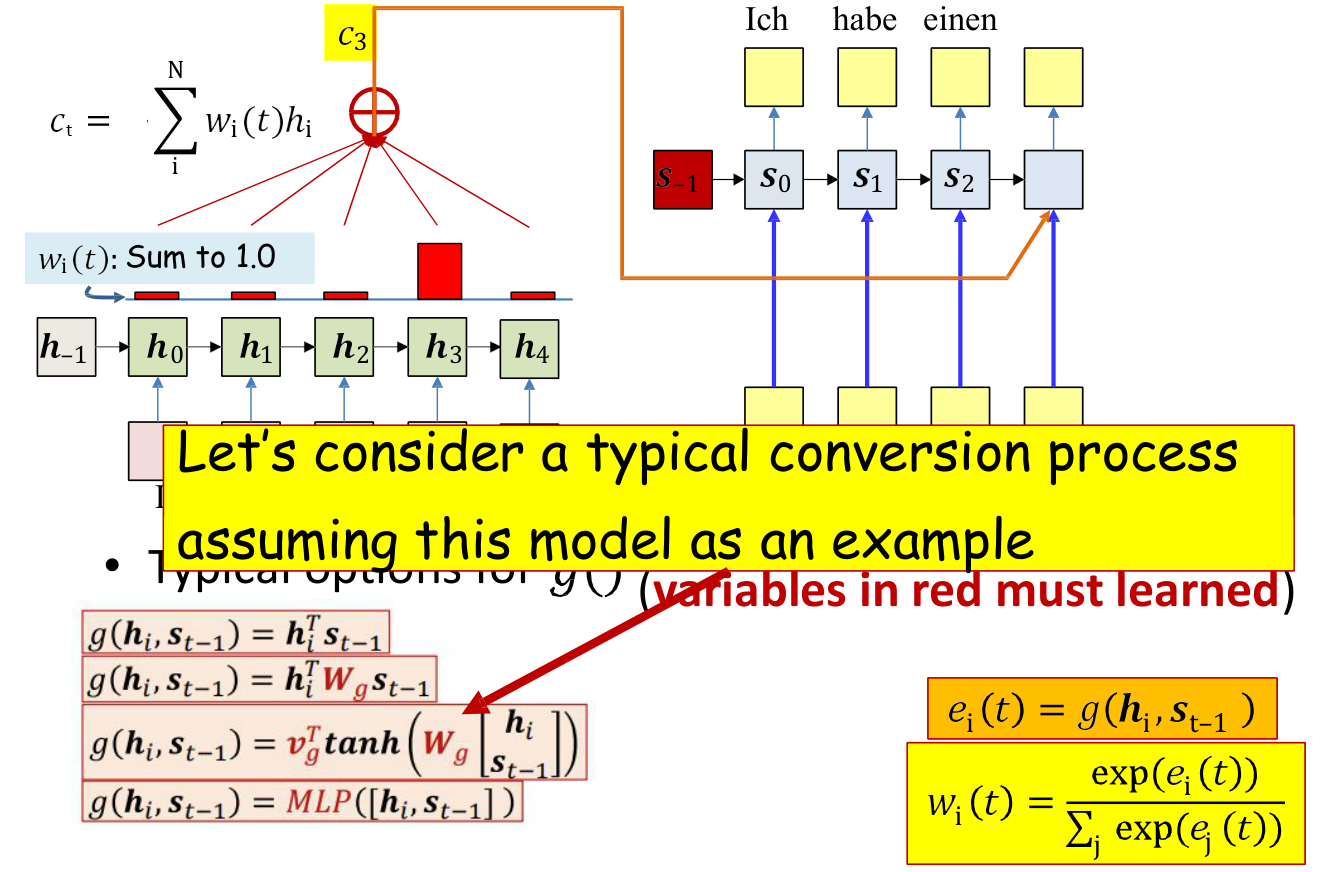
\includegraphics[width=0.8\paperwidth,height=0.72\paperheight,keepaspectratio]{images/seq2seq+attention/seq2seq_attention_conversion_example.png}

  {\scriptsize Source: after CMU 11-785 (Spring 2024), Lecture 18: Sequence to Sequence Models \& Attention, slide~36.}
\end{frame}

\begin{frame}{Converting an input: Inference}
  \centering
  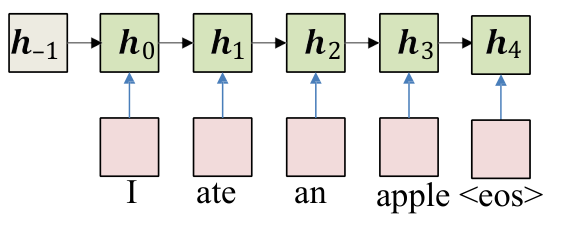
\includegraphics[width=0.4\paperwidth,height=0.4\paperheight,keepaspectratio]{images/seq2seq+attention/seq2seq_encoder_hidden_states_only.png}

  {\scriptsize Source: after CMU 11-785 (Spring 2024), Lecture 18: Sequence to Sequence Models \& Attention, slide~37.}
  \begin{itemize}
    \item[] \textbf{Pass the input through the encoder to produce hidden representations $\pmb{h_i}$}
  \end{itemize}
\end{frame}

\begin{frame}{Converting an input: Inference}
  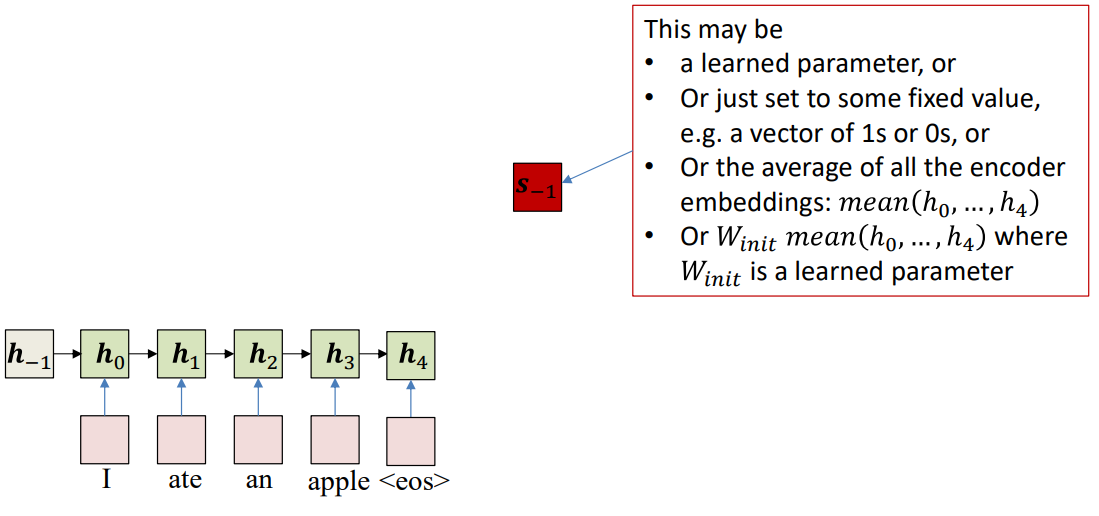
\includegraphics[width=0.6\paperwidth,height=0.6\paperheight,keepaspectratio]{images/seq2seq+attention/seq2seq_decoder_initial_state_options.png}

  {\scriptsize Source: after CMU 11-785 (Spring 2024), Lecture 18: Sequence to Sequence Models \& Attention, slide~38.}
  \begin{itemize}
    \item[] \textbf{Pass the input through the encoder to produce hidden representations $\pmb{h_i}$}
  \end{itemize}
\end{frame}

\begin{frame}{Converting an input: Inference}
  \centering
  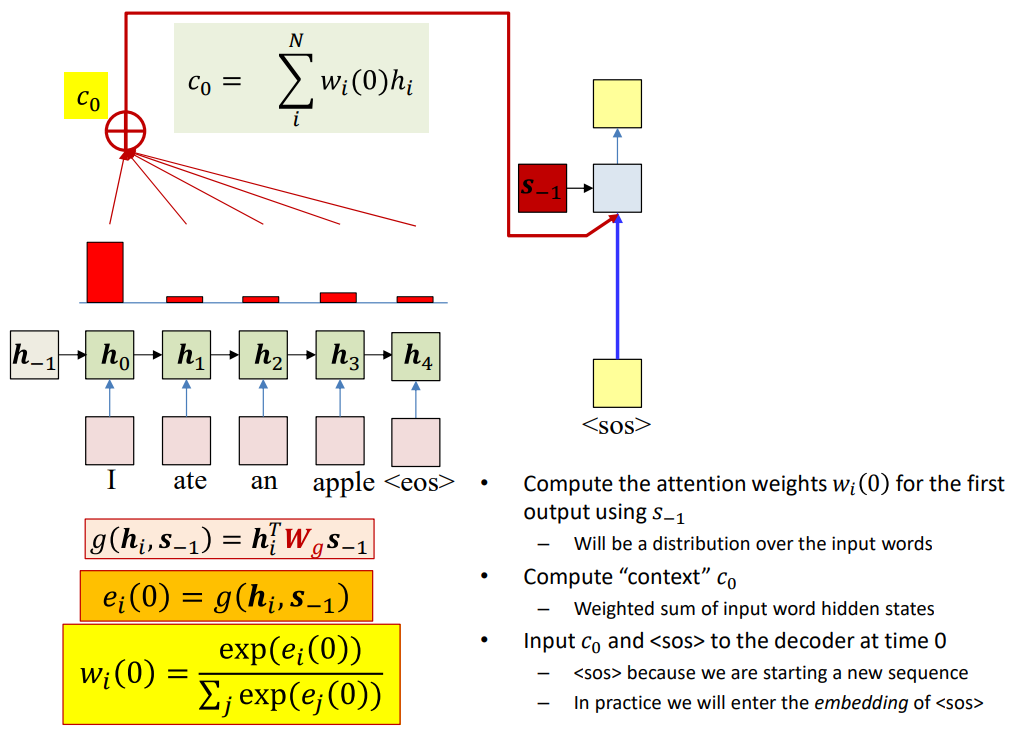
\includegraphics[width=0.8\paperwidth,height=0.72\paperheight,keepaspectratio]{images/seq2seq+attention/seq2seq_attention_first_context_c0.png}

  {\scriptsize Source: after CMU 11-785 (Spring 2024), Lecture 18: Sequence to Sequence Models \& Attention, slide~39.}
\end{frame}

\begin{frame}{Converting an input: Inference}
  \centering
  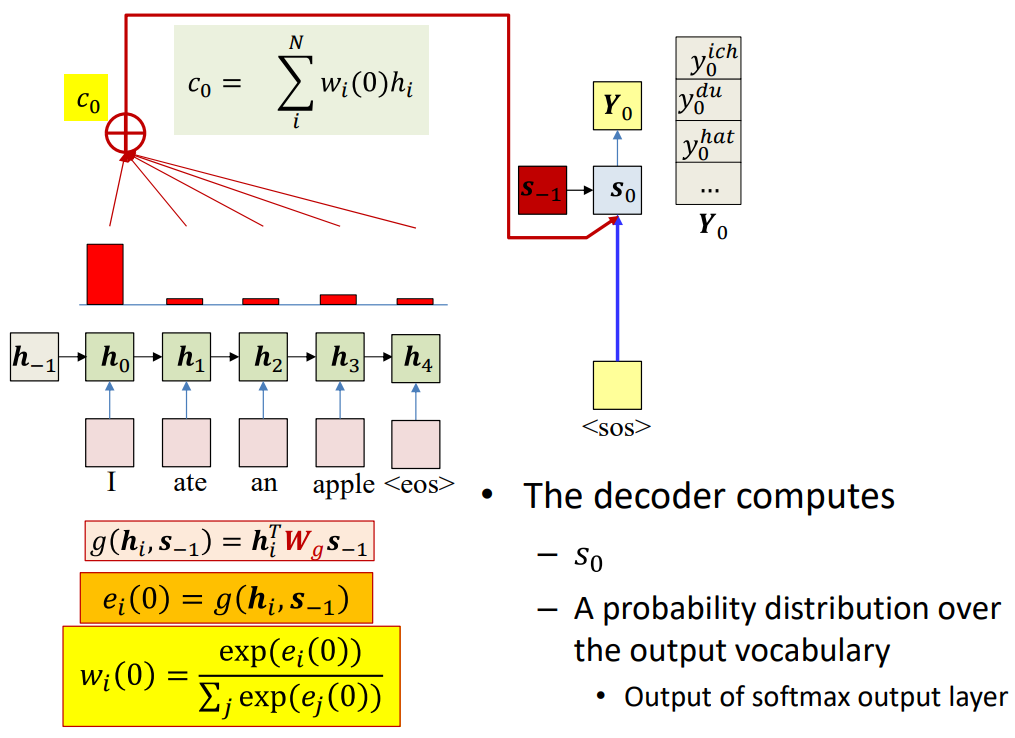
\includegraphics[width=0.8\paperwidth,height=0.72\paperheight,keepaspectratio]{images/seq2seq+attention/seq2seq_decoder_first_output_distribution.png}

  {\scriptsize Source: after CMU 11-785 (Spring 2024), Lecture 18: Sequence to Sequence Models \& Attention, slide~40.}
\end{frame}

\begin{frame}{Converting an input: Inference}
  \centering
  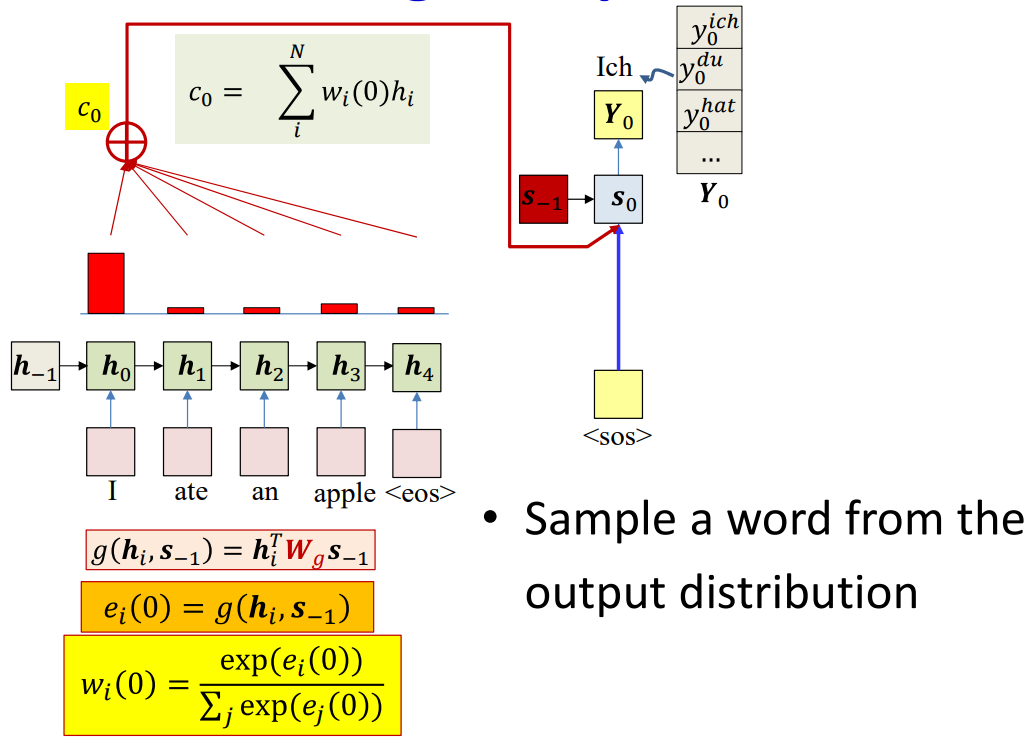
\includegraphics[width=0.8\paperwidth,height=0.72\paperheight,keepaspectratio]{images/seq2seq+attention/seq2seq_decoder_sample_first_word.png}

  {\scriptsize Source: after CMU 11-785 (Spring 2024), Lecture 18: Sequence to Sequence Models \& Attention, slide~41.}
\end{frame}

\begin{frame}{Converting an input: Inference}
  \centering
  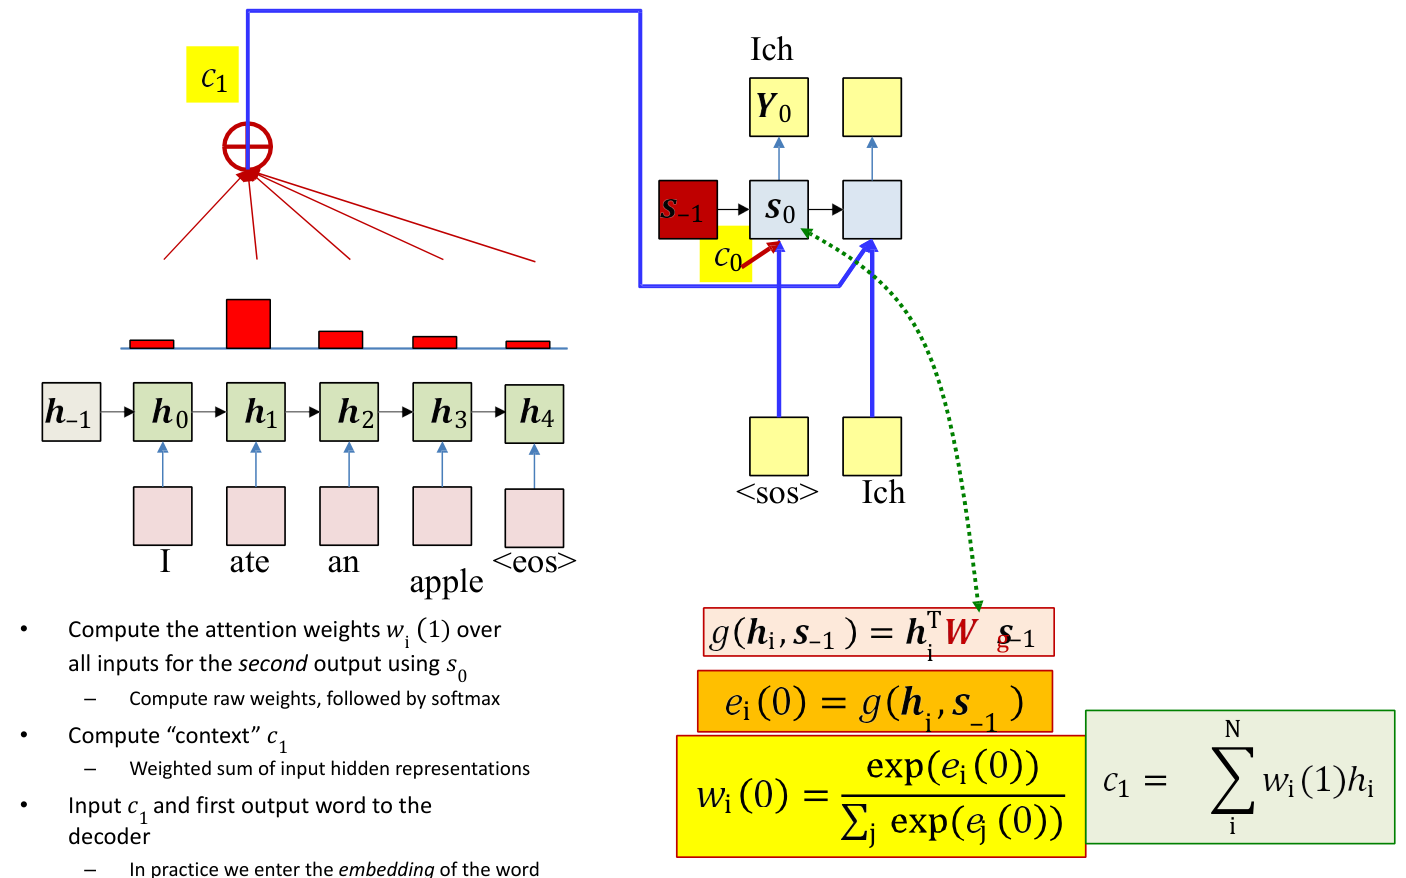
\includegraphics[width=0.8\paperwidth,height=0.72\paperheight,keepaspectratio]{images/seq2seq+attention/seq2seq_attention_second_context_c1.png}

  {\scriptsize Source: after CMU 11-785 (Spring 2024), Lecture 18: Sequence to Sequence Models \& Attention, slide~42.}
\end{frame}

\begin{frame}{Converting an input: Inference}
  \centering
  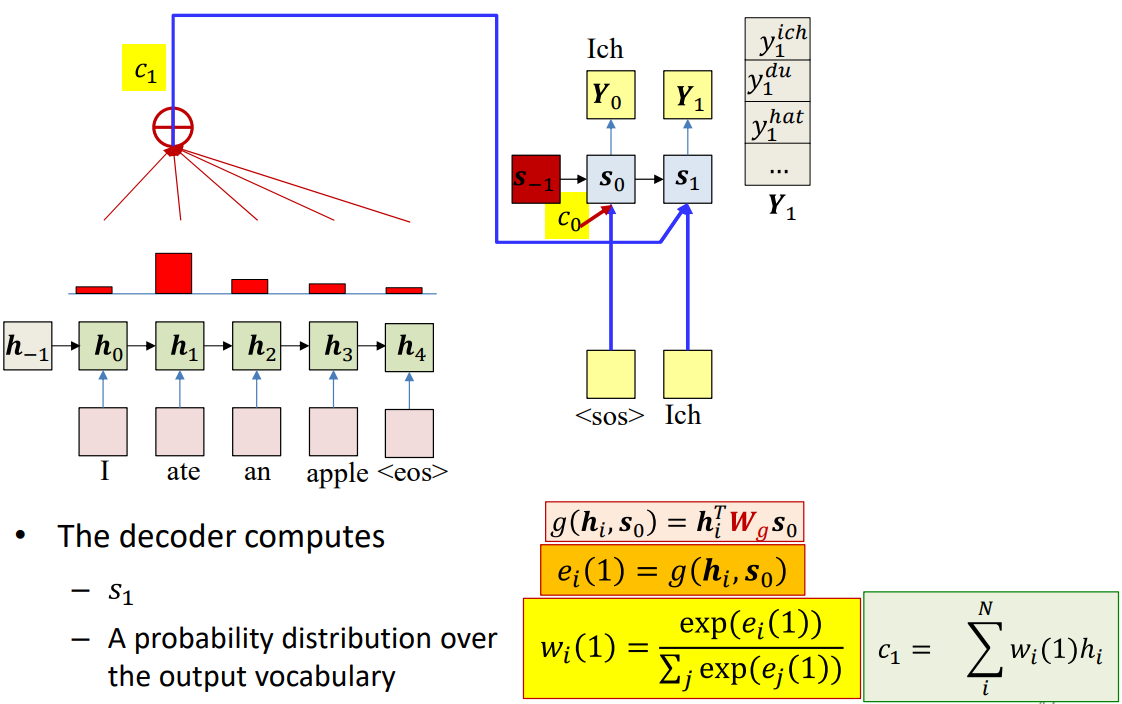
\includegraphics[width=0.8\paperwidth,height=0.72\paperheight,keepaspectratio]{images/seq2seq+attention/seq2seq_decoder_second_output_distribution.png}

  {\scriptsize Source: after CMU 11-785 (Spring 2024), Lecture 18: Sequence to Sequence Models \& Attention, slide~43.}
\end{frame}

\begin{frame}{Converting an input: Inference}
  \centering
  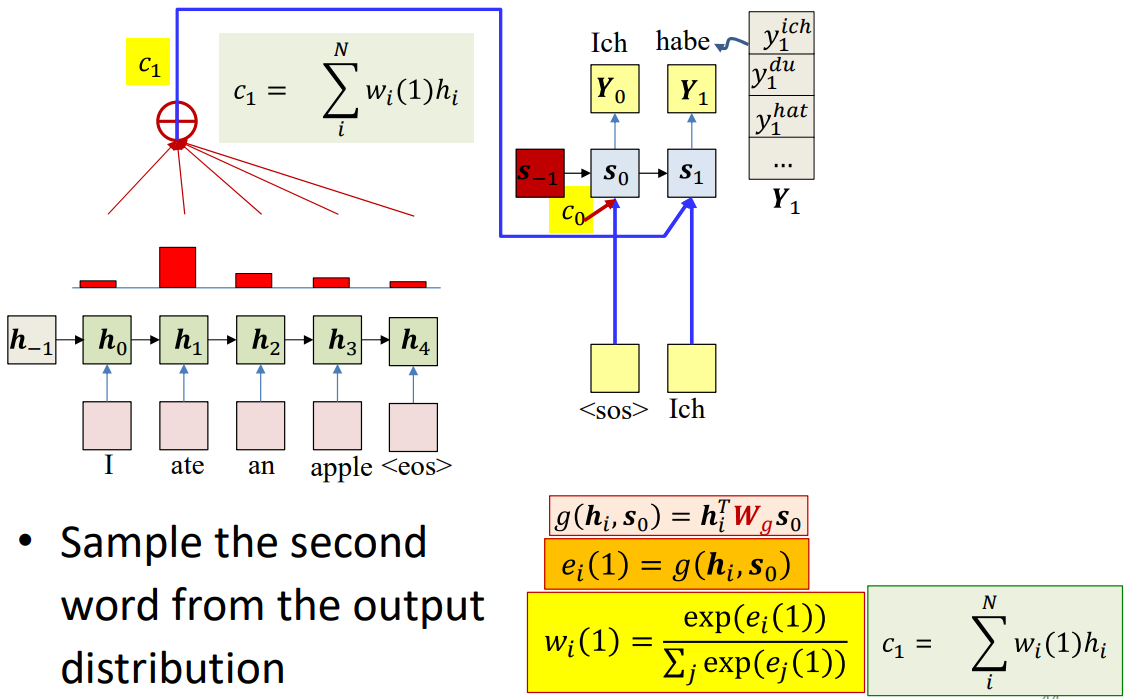
\includegraphics[width=0.8\paperwidth,height=0.72\paperheight,keepaspectratio]{images/seq2seq+attention/seq2seq_decoder_sample_second_word.png}

  {\scriptsize Source: after CMU 11-785 (Spring 2024), Lecture 18: Sequence to Sequence Models \& Attention, slide~44.}
\end{frame}

\begin{frame}{Converting an input: Inference}
  \centering
  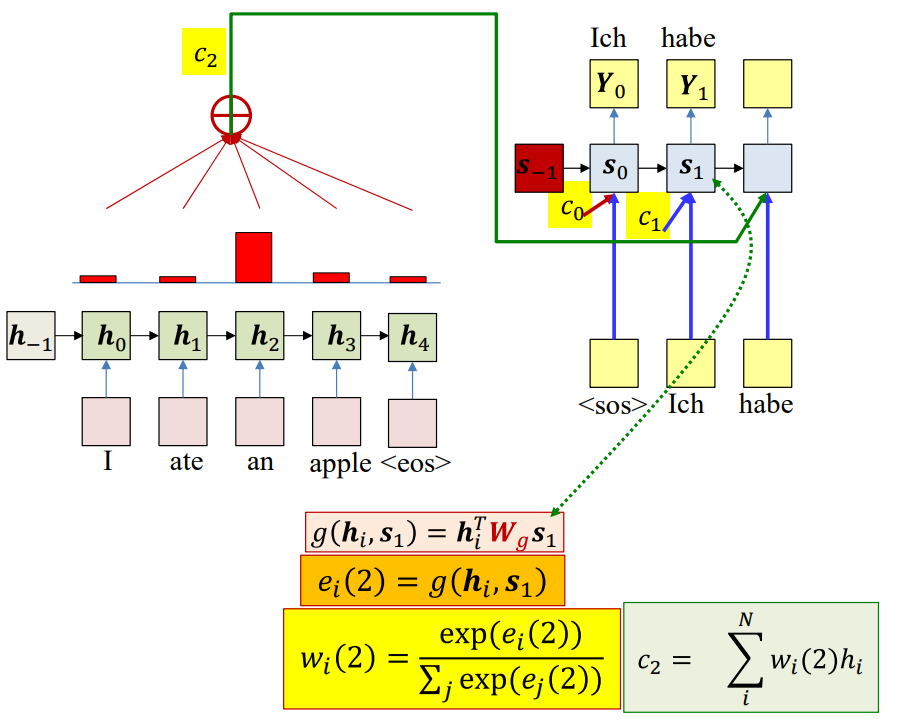
\includegraphics[width=0.8\paperwidth,height=0.72\paperheight,keepaspectratio]{images/seq2seq+attention/seq2seq_attention_third_context_c2.png}

  {\scriptsize Source: after CMU 11-785 (Spring 2024), Lecture 18: Sequence to Sequence Models \& Attention, slide~45.}
\end{frame}

\begin{frame}{Converting an input: Inference}
  \centering
  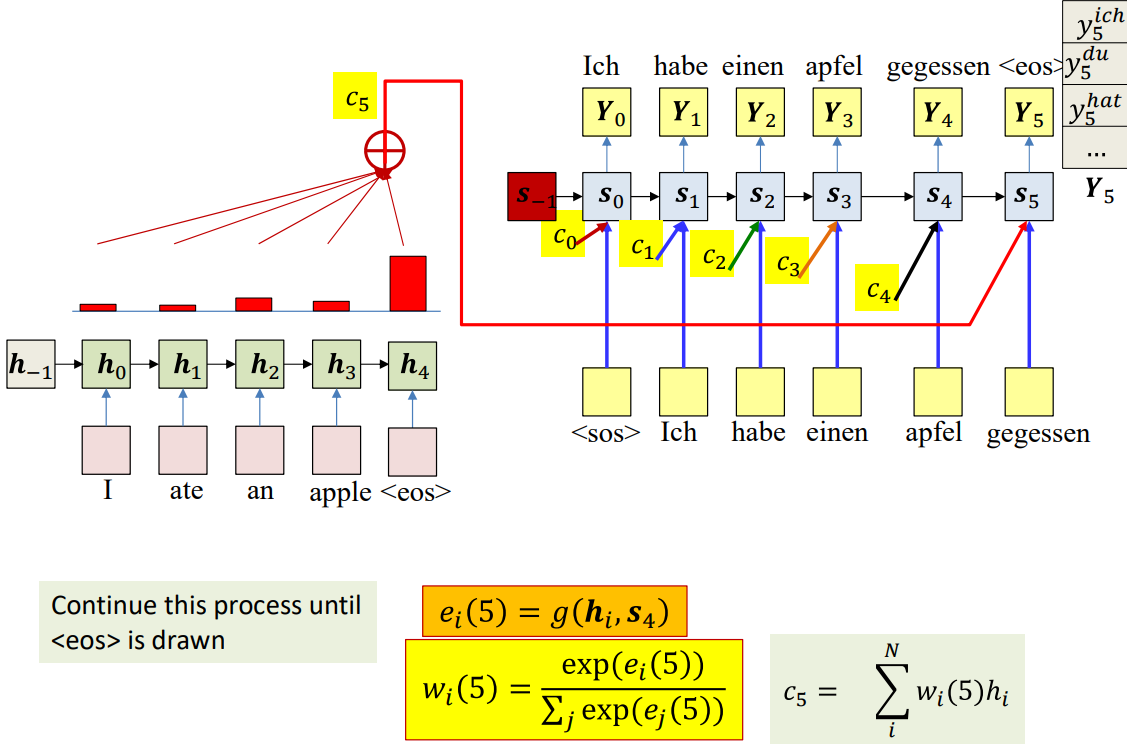
\includegraphics[width=0.8\paperwidth,height=0.72\paperheight,keepaspectratio]{images/seq2seq+attention/seq2seq_attention_final_step_c5.png}

  {\scriptsize Source: after CMU 11-785 (Spring 2024), Lecture 18: Sequence to Sequence Models \& Attention, slide~56.}
\end{frame}

\begin{frame}{Attention-based Decoding}
  \centering
  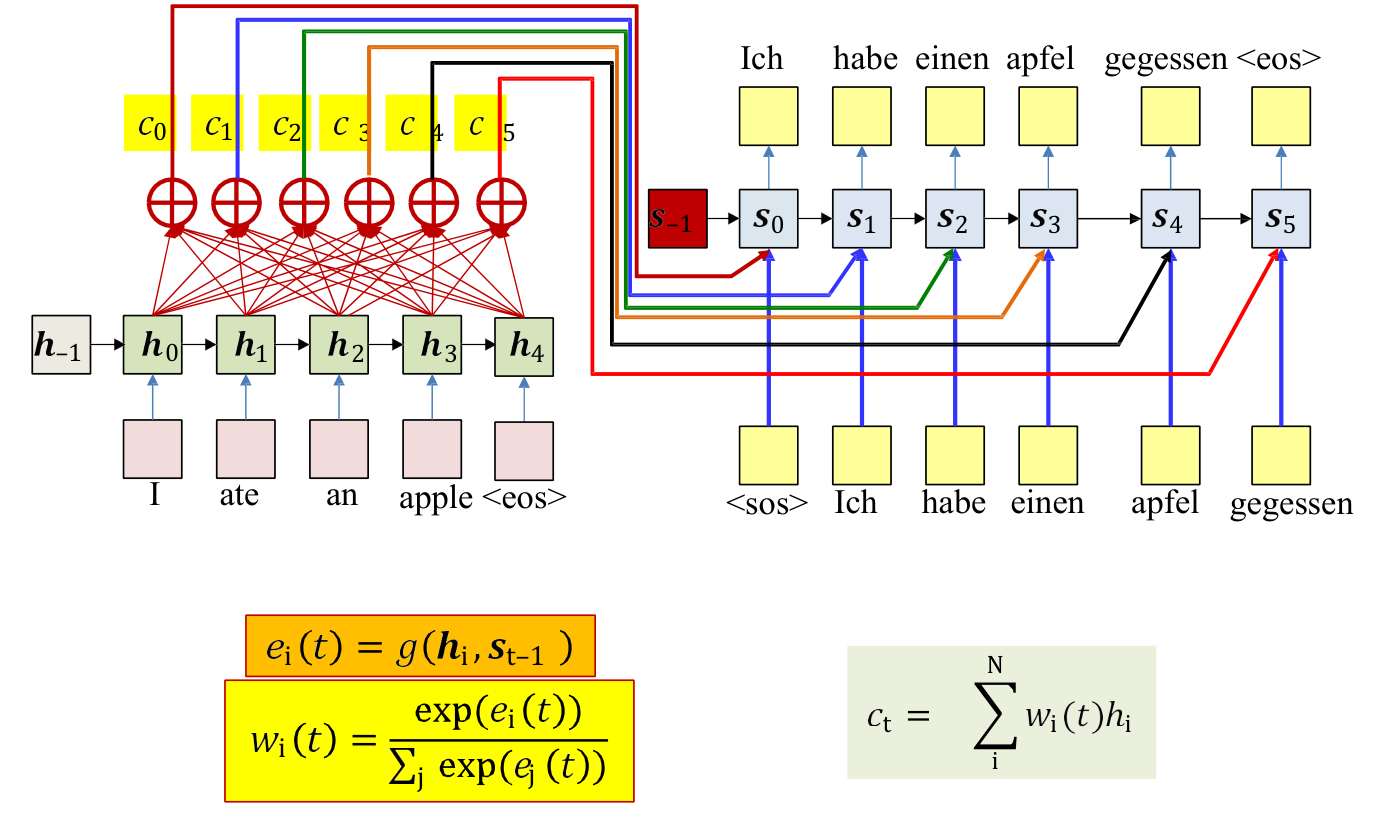
\includegraphics[width=0.8\paperwidth,height=0.72\paperheight,keepaspectratio]{images/seq2seq+attention/seq2seq_attention_all_contexts_summary.png}

  {\scriptsize Source: after CMU 11-785 (Spring 2024), Lecture 18: Sequence to Sequence Models \& Attention, slide~57.}
\end{frame}

\begin{frame}{Recap: Sequence to Sequence Models}
  \centering
  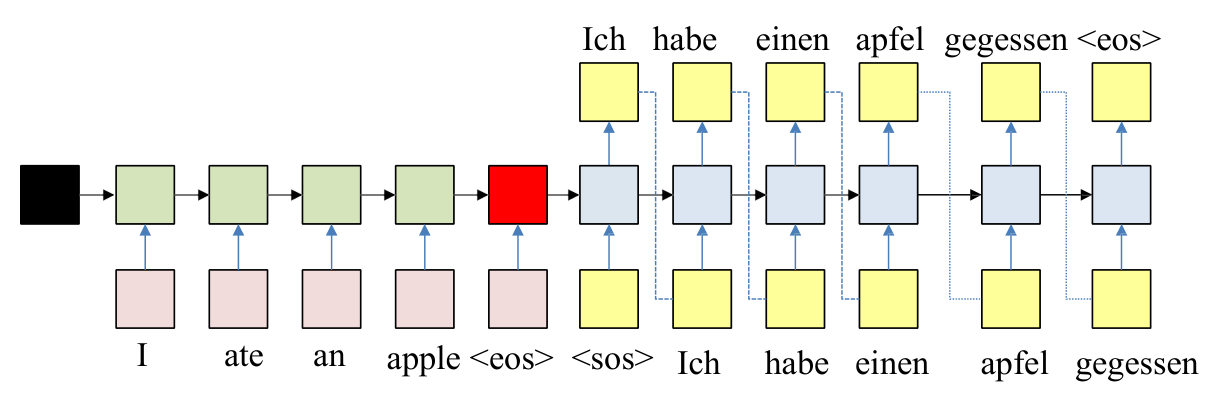
\includegraphics[width=0.4\paperwidth,height=0.4\paperheight,keepaspectratio]{images/seq2seq+attention/seq2seq_decoder_teacher_forcing.png}

  {\scriptsize Source: after CMU 11-785 (Spring 2024), Lecture 18: Sequence to Sequence Models \& Attention, slide~98.}
\begin{itemize}
  \item The input sequence feeds into a recurrent structure
  \item The input sequence is terminated by an explicit \textless eos\textgreater{} symbol
    \begin{itemize}
      \item \textcolor{red}{The hidden activation at the \textless eos\textgreater{} ``stores'' all information about the sentence}
    \end{itemize}
  \item Subsequently a second RNN uses the hidden activation as initial state to produce a sequence of outputs
\end{itemize}
\end{frame}

\begin{frame}{Recap: Attention Models}
  \centering
  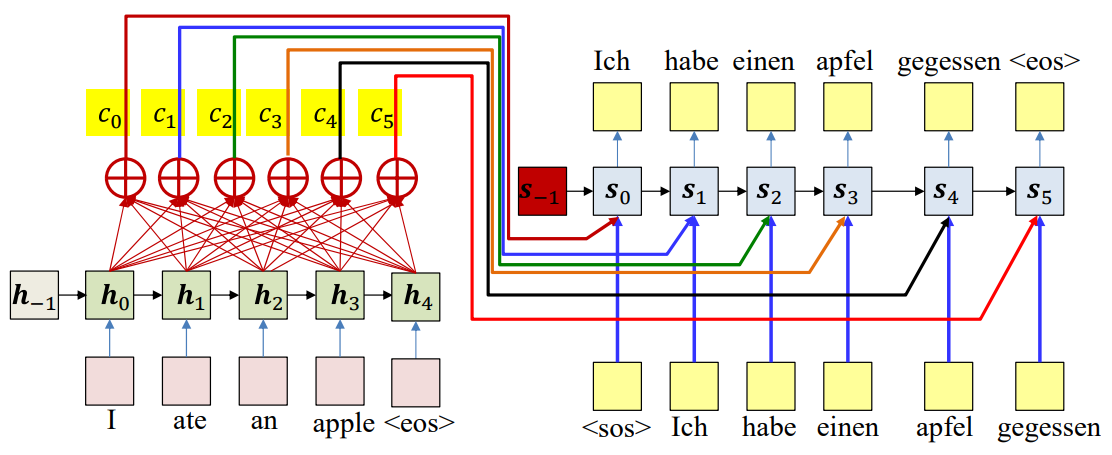
\includegraphics[width=0.4\paperwidth,height=0.4\paperheight,keepaspectratio]{images/seq2seq+attention/seq2seq_attention_all_contexts_distinct.png}

  {\scriptsize Source: after CMU 11-785 (Spring 2024), Lecture 18: Sequence to Sequence Models \& Attention, slide~99.}
\begin{itemize}
  \item Encoder recurrently produces hidden representations of input word sequence
  \item Decoder recurrently generates output word sequence
    \begin{itemize}
      \item For each output word the decoder uses a weighted average of the hidden input representations as input ``context'', along with the recurrent hidden state and the previous output word
    \end{itemize}
\end{itemize}
\end{frame}

\begin{frame}{Recap: Attention Models}
  \centering
  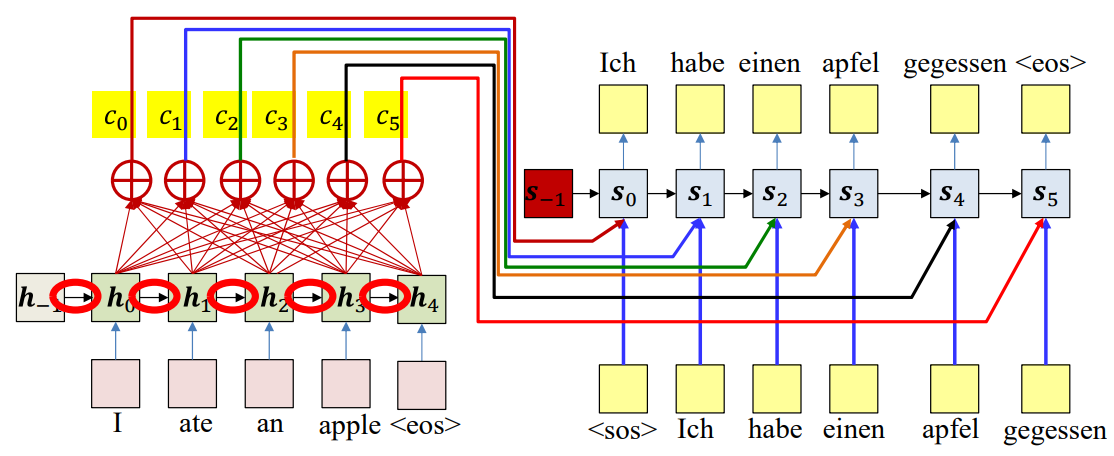
\includegraphics[width=0.4\paperwidth,height=0.4\paperheight,keepaspectratio]{images/seq2seq+attention/seq2seq_attention_backprop_through_encoder.png}

  {\scriptsize Source: after CMU 11-785 (Spring 2024), Lecture 18: Sequence to Sequence Models \& Attention, slide~100.}
\begin{itemize}
  \item \textbf{Problem:} Because of the recurrence, the hidden representation for any word is also influenced by \emph{all} preceding words
    \begin{itemize}
      \item The decoder is actually paying attention to the sequence, and not just the word
    \end{itemize}
\end{itemize}
\end{frame}
